
Sau khi hoàn thiện các khối chức năng riêng biệt, bước cuối cùng là tích hợp chúng vào một module duy nhất gọi là \texttt{CPU\_Top}. Module này đóng vai trò là khung xương kết nối các đường bus dữ liệu, bus địa chỉ và các tín hiệu điều khiển giữa các khối thành phần theo kiến trúc máy tính đã thiết kế.

\textbf{ Mã nguồn Verilog hiện thực module CPU\_Top:}

\begin{lstlisting}[language=Verilog, caption={Ma nguon hien thuc module tich hop he thong Top-level}]
module CPU_Top (
    input clk,
    input rst,
    output halt // Tin hieu bao dung he thong
);
    // Cac duong day ket noi noi bo (Internal Signals)
    wire [31:0] bus_data;      // Bus du lieu chung (inout)
    wire [31:0] addr_to_mem;   // Dia chi gui den Memory
    wire [31:0] pc_to_mux;     // Dia chi tu PC
    wire [31:0] alu_out;       // Ket qua tu ALU
    wire [31:0] acc_out;       // Du lieu tu Accumulator (inA cua ALU)
    
    wire [2:0] opcode;         // Ma lenh tu IR gui den Controller/ALU
    wire [28:0] ir_addr_part;  // Phan dia chi cua lenh
    wire is_zero;              // Co zero tu ALU
    
    // Cac tin hieu dieu khien tu Controller
    wire sel, rd, wr, ld_ir, ld_ac, ld_pc, inc_pc, data_e;

    // 1. Khoi Program Counter (PC)
    program_counter PC (
        .clk(clk), .rst(rst), .ld_pc(ld_pc), .inc_pc(inc_pc),
        .d_in({3'b000, ir_addr_part}), .pc_out(pc_to_mux)
    );

    // 2. Khoi Address Mux
    address_mux #(.WIDTH(32)) AddrMux (
        .pc_addr(pc_to_mux), .ir_addr({3'b000, ir_addr_part}),
        .sel(sel), .addr_out(addr_to_mem)
    );

    // 3. Khoi Instruction Register (IR)
    instruction_reg IR (
        .clk(clk), .rst(rst), .ld_ir(ld_ir),
        .data_in(bus_data), .opcode(opcode), .addr(ir_addr_part)
    );

    // 4. Khoi dieu khien trung tam (Controller)
    controller ControlUnit (
        .clk(clk), .rst(rst), .opcode(opcode), .is_zero(is_zero),
        .sel(sel), .rd(rd), .ld_ir(ld_ir), .halt(halt),
        .inc_pc(inc_pc), .ld_ac(ld_ac), .ld_pc(ld_pc),
        .wr(wr), .data_e(data_e)
    );

    // 5. Khoi ALU
    ALU MainALU (
        .inA(acc_out), .inB(bus_data), .opcode(opcode),
        .out(alu_out), .is_zero(is_zero)
    );

    // 6. Khoi thanh ghi tich luy (Accumulator)
    Accumulator ACC (
        .clk(clk), .rst(rst), .load_en(ld_ac),
        .D(alu_out), .Q(acc_out)
    );

    // 7. Khoi Bo nho (Memory)
    memory RAM (
        .clk(clk), .addr(addr_to_mem),
        .rd(rd), .wr(wr), .data(bus_data)
    );

    // 8. Dieu khien Bus du lieu (Tri-state buffer)
    // Khi lenh STO thuc thi, dua du lieu tu ACC ra Bus de ghi vao RAM
    assign bus_data = (data_e) ? acc_out : 32'bz;

endmodule
\end{lstlisting}

\textbf{Mô tả cơ chế kết nối và vận hành:}
\begin{itemize}
    \item \textbf{Cấu trúc Bus chung:} Module sử dụng một đường \texttt{bus\_data} song hướng duy nhất để kết nối giữa \textit{Memory}, \texttt{IR} và \texttt{ALU}. Cơ chế \textit{Tri-state buffer} được áp dụng tại dòng lệnh \texttt{assign bus\_data} nhằm đảm bảo dữ liệu chỉ được đẩy từ CPU ra bộ nhớ khi lệnh \texttt{STO} (Store) được thực thi.
    
    \item \textbf{Phân luồng địa chỉ:} Thông qua khối \texttt{address\_mux}, hệ thống linh hoạt chuyển đổi giữa địa chỉ nạp lệnh (từ \texttt{PC}) và địa chỉ dữ liệu (từ \texttt{IR}) tùy theo pha của chu kỳ lệnh. Trong quá trình kết nối, địa chỉ toán hạng được trích xuất từ \textit{Instruction Register} (\texttt{ir\_addr\_part}) có độ rộng 29-bit. Nhóm thực hiện phép ghép bit (\textit{concatenation}) để mở rộng về đúng 32-bit:

    \begin{center}
    \begin{tabular}{|l|}
    \hline
    \texttt{\{3'b000, ir\_addr\_part\} // 3-bit 0 + 29-bit địa chỉ = 32-bit} \\
    \hline
    \end{tabular}
    \end{center}

    Ba bit \texttt{3'b000} được ghép vào phần cao nhất nhằm đảm bảo giá trị địa chỉ được \textit{zero-extend}. Điều này đảm bảo:
    \begin{itemize}
        \item \textbf{Tính đúng đắn về giá trị:} Địa chỉ \texttt{29'h10} trở thành \texttt{32'h00000010}, trỏ đúng vào ô nhớ số 16.
        \item \textbf{Tránh lỗi tổng hợp:} Vivado yêu cầu các tín hiệu phải khớp hoàn toàn về độ rộng bit để tránh lỗi kết nối không tương thích.
    \end{itemize}

    Cơ chế này cũng áp dụng cho lệnh \textbf{JMP}:
    \begin{center}
    \begin{tabular}{|l|}
    \hline
    \texttt{.d\_in(\{3'b000, ir\_addr\_part\}) // Địa chỉ đích JMP -> PC} \\
    \hline
    \end{tabular}
    \end{center}

    \item \textbf{Vòng lặp Phản hồi (Feedback Loop):} Tín hiệu \texttt{is\_zero} từ \texttt{ALU} được gửi ngược về \textit{Controller} để xử lý lệnh rẽ nhánh \texttt{SKZ}.
\end{itemize}

\begin{figure}[H]
    \centering
    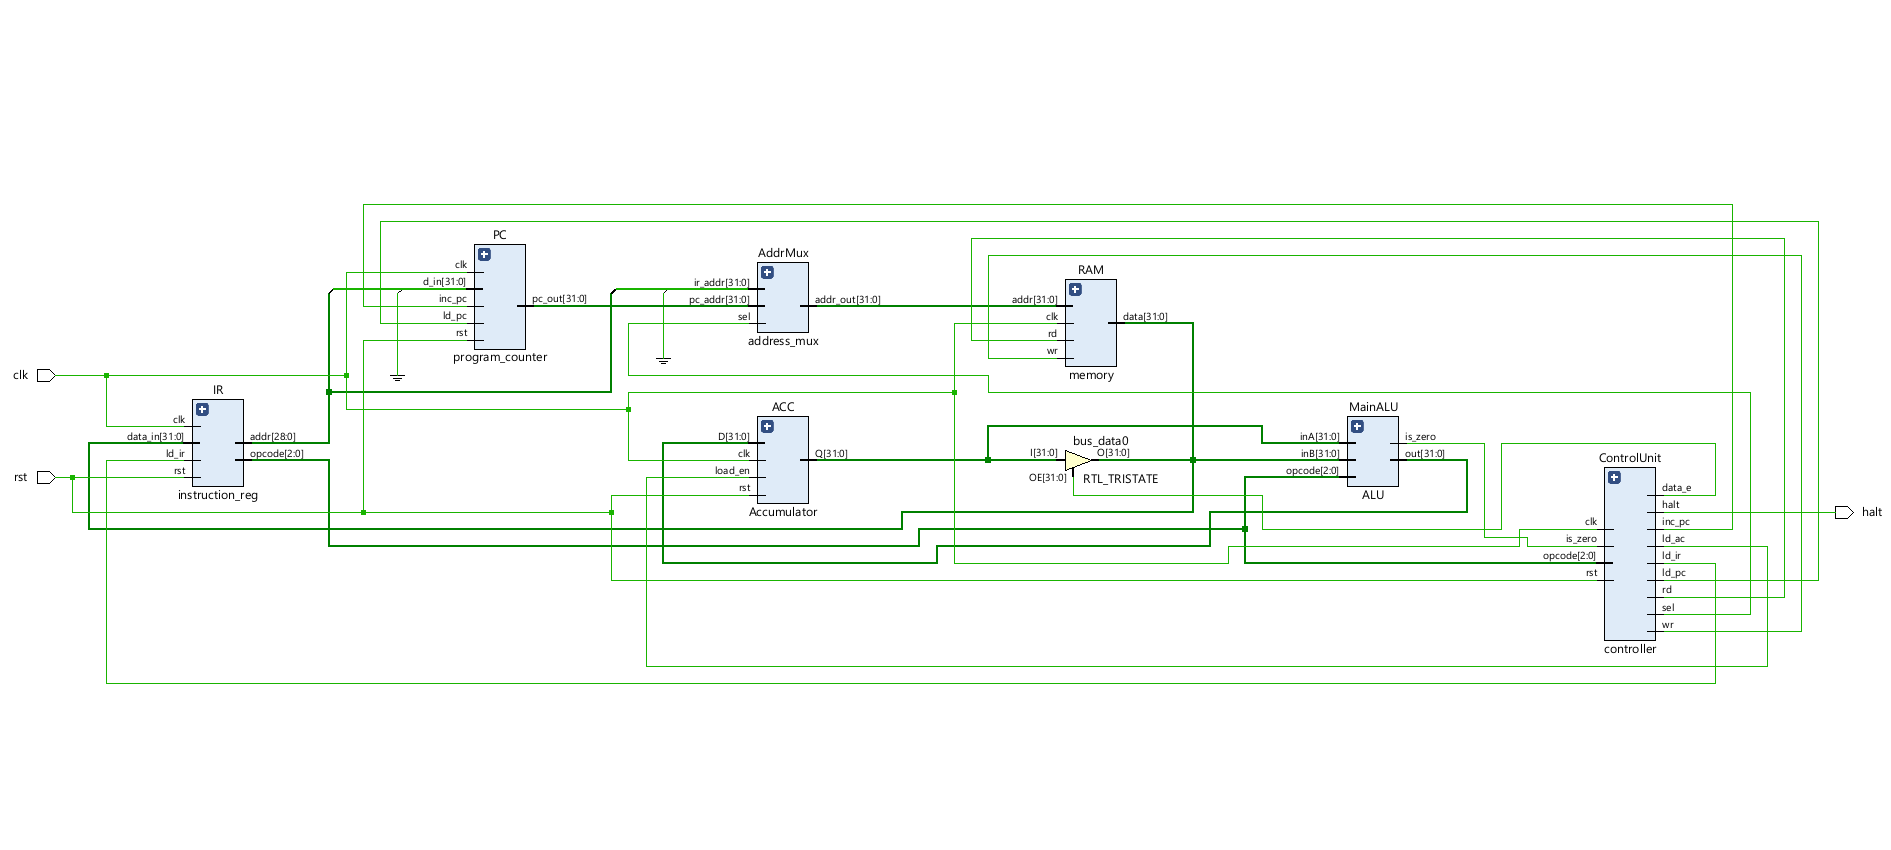
\includegraphics[width=0.9\textwidth]{sodocpu.png} 
    \caption{Sơ đồ mạch tích hợp hệ thống CPU (RTL Schematic)}
    \label{fig:cpu_top_rtl}
\end{figure}